\subsection[ZipSessionKit]{ZipSessionKit \hyperref[zipSessionPb]{$\uparrow$}}
\label{zipSessionSol}

Pour pouvoir répondre aux objectifs notre PIDR, nous avons décidé de développer un nouveau SessionKit. Cette nouvelle implémentation nous permettra de stocker les progrès des élèves de manière locale d'une manière plus simple. Nous aurons également plus facilement accès au code de chaque exercice. Pour cela, en accord avec Martin Quinson et Gérald Oster, nous avons choisi d'utiliser comme solution technique Git car cela permettrait de s'affranchir au maximum d'une technologie qui aurait pu être trop spécifique. En effet, Git est utilisé par 40 \%\cite{GitUsage} des programmeurs et est un outil qui est fait pour durer et dont les bases ne sont pas prêtes de changer dans les années à venir. Étant donné qu'il a été créé à l'origine pour pouvoir gérer le développement du noyau Linux, il est stable et performant. La gestion de version offerte par Git pourrait également permettre un retour en arrière facile pour permettre aux enseignants de visualiser les différentes étapes du code de l'élève lors de son raisonnement pour résoudre le problème posé. À terme, cela pourrait même être utilisé pour permettre à l'élève de revenir en arrière simplement dans son code.


Le code de l'utilisateur est alors sauvegardé à chaque fois qu'il teste ou change d'exercice. Il est en fait mis dans un commit\footnote{Sauvegarde des fichiers à un instant t.} dont le message associé est formaté en JSON\footnote{Format de données textuelles, générique, qui permet de représenter de l'information structurée.}. Il contient :
\begin{itemize}
\item le type d'évènement ;
\item le langage utilisé ;
\item l'exercice courant ;
\item le nombre de tests de l'exercice courant ;
\item le nombre de tests satisfaits par le code de l'utilisateur.
\end{itemize}

$ $

\begin{lstlisting}[language = plm,basicstyle={\footnotesize\ttfamily}, caption= Message de commit]
{"os":"Windows 8 (version: 6.2; arch: amd64)","plm_version":"2.3beta (20140125)","evt_type":"started","java_version":"1.7.0_51 (VM: Java HotSpot(TM) 64-Bit Server VM; version: 24.51-b03)","start_date":"2014\/05\/21 13:08:26"}

{"course":"","exolang":"Java","exoswitchto":"The small cousines of Buggles","evt_type":"switched","totaltests":"-1","passedtests":"0","exoname":"The small cousines of Buggles"}
\end{lstlisting}

$ $

Le commit contient d'autres fichiers que le code de l'élève. En effet, l'énoncé peut être amené à être modifié, c'est pourquoi nous le conservons aussi ainsi que la correction associée. Cela permettra également aux professeurs qui regardent un commit en particulier de connaître le contexte et l'énoncé à l'instant t où l'élève a fait tel exercice. 
Un fichier contenant les erreurs de compilation du code de l'utilisateur est aussi sauvegardé.


Les commits sont gérés par une classe GitSpy qui implémente \texttt{ProgressSpyListener}. Elle récupère des évènements de type :
\begin{itemize}
\item démarrage de la PLM ;
\item exécution du code ;
\item changement d'exercice.
\end{itemize}

Utiliser Git pourra également nous permettre de gérer facilement plusieurs utilisateurs sur une même machine, à partir du moment où nous utilisons une branche spécifique pour chaque utilisateur. Voir la figure~\ref{gitLocal}.

\begin{figure}[!h]
\begin{center}
	\begin{tikzpicture}
\node[server](PC1) at (-3,0) {};
\node[xshift=-0.8cm,yshift=0.2cm,left of = PC1,align=left](PC1label) {Utilisateurs A};

\node(GitA1) at (-5.5,-2) {
\includegraphics[scale=0.25]{images/git.ps}}; 
\node[below of = GitA1,align=left](GitAlabel1) {Git local utilisateur A1};

\node(GitA2) at (-0.5,-2) {
\includegraphics[scale=0.25]{images/git.ps}}; 
\node[below of = GitA2,align=left](GitAlabel1) {Git local utilisateur A2};

\draw[thick,darkgray!10!gray] (PC1.south east)--(GitA1);
\draw[thick,darkgray!10!gray] (PC1.south west)--(GitA2);
\end{tikzpicture}

    \caption{Git locaux}
    \label{gitLocal}
\end{center}
\end{figure}

\subsection[Serveur distant]{Serveur distant \hyperref[serveurDistantPb]{$\uparrow$}}
\label{serveurDistantSol}

Une fois les données des utilisateurs mis en forme dans un dépôt Git local, il faut que les professeurs puissent y accéder facilement. Nous avons donc décidé assez logiquement d'utiliser un serveur Git distant puisque nous n'aurions alors qu'à pusher les modifications locales. Ce dépôt central devra contenir le code de tous les utilisateurs de la PLM. Pour ne pas que le code des différents usagers se mélange, nous avons décider d'utiliser une branche par personne. Chaque fois que le code sera envoyé sur le dépôt central, il sera envoyé dans une branche spécifique. Comme il n'est pas forcément possible ni très sécurisé de permettre à n'importe qui de pusher anonynement dans un dépôt Git distant, nous avons préféré lors de nos tests créer un dépôt sur Bitbucket\cite{depotBitbucket} avec un compte utilisateur créé dans le seul but de permettre à la PLM d'y pusher du code. Les identifiants de ce compte utilisateur sont stockés dans la PLM. Voir la la figure~\ref{fig:gitDistant}.

\begin{figure}[!h]
\begin{center}
	
\begin{tikzpicture}[scale=0.5, every node/.style={scale=0.6}]
\node[server](PC1) at (-3,-1) {};
\node[xshift=-0.8cm,yshift=0.2cm,left of = PC1,align=left](PC1label) {Utilisateurs A};

\node(GitA1) at (-5,-2.5) {
\includegraphics[scale=0.25]{images/git.ps}}; 
\node[below of = GitA1,align=left](GitAlabel1) {Git local A1};

\node(GitA2) at (-2,-2.5) {
\includegraphics[scale=0.25]{images/git.ps}}; 
\node[below of = GitA2,align=left](GitAlabel2) {Git local A2};

\node[server](PC2) at (3,-1) {};
\node[xshift=-0.8cm,yshift=0.2cm,left of = PC2,align=left](PC2label) {Utilisateur B};

\node(GitB) at (3,-2.5) {
\includegraphics[scale=0.25]{images/git.ps}}; 
\node[xshift=-0.5cm,left of = GitB,align=left](GitBlabel) {Git local B};
\node[red,inner sep=0mm](croix) at (1.3,0.8) {\begin{LARGE}$\times$\end{LARGE}};

\node[server](PC3) at (4.5,0.5) {};
\node[xshift=0.6cm,right of = PC3,align=left](PC3label) {Utilisateur C};

\node(GitC) at (5.5,-0.5) {
\includegraphics[scale=0.25]{images/git.ps}}; 
\node[xshift=0.7cm,right of = GitC,align=left](GitClabel) {Git local C};


\node[my cloud, minimum width=1.25cm, minimum height=1.55cm,font=\large] (cloud) at (0,2) {Internet};

\node(Git) at (-3.5,3) {
\includegraphics[scale=0.5]{images/git.ps}}; 
\node[xshift=-1cm,left of = Git,align=left](Gitlabel) {Git central};


\draw[thick,darkgray!10!gray] (PC1.north west)--(cloud);
\draw[thick,darkgray!10!gray] (PC1.south east)--(GitA1);
\draw[thick,darkgray!10!gray] (PC1.south west)--(GitA2);
\draw[thick,darkgray!10!gray] (PC2.north east)--(1.3,0.8);
\draw[thick,darkgray!10!gray] (PC2.south)--(GitB);
\draw[thick,darkgray!10!gray] (PC3.north east)--(cloud);
\draw[thick,darkgray!10!gray] (PC3.south)--(GitC);
\draw[thick,darkgray!10!gray] (Git.east)--(cloud);
\path[<->, blue,line width = 0.5mm] (GitA2)  edge   [bend left=-80]   node {} (Git.east);

\path[<->, blue,line width = 0.5mm] (0,-5)  edge [auto]  node {Git push/pull} (2.5,-5);

\end{tikzpicture}

    \caption{Avec un dépôt Git central}
	\label{fig:gitDistant}
\end{center}
\end{figure}

\subsection[Anonymat des données]{Anonymat des données \hyperref[anonymatPb]{$\uparrow$}}
\label{anonymatSol}

Le code écrit par tous les utilisateurs est disponible sur le dépôt Git central. Ceci nous permet de proposer aux utilisateurs de continuer une session entamée sur une autre machine. Pour cela, nous générons et donnons un identifiant unique à l'utilisateur. Celui-ci sert de mot de passe pour continuer sa session sur une autre machine. Cet identifiant est généré par Java grâce à la classe UUID\cite{UUID}. Il fait 128 bits de long et est créé à partir de la date et d'une partie générée aléatoirement. La probabilité d'une collision est très faible\cite{ietfUUID}. Cet identifiant peut donc être demandé au lancement de la PLM pour continuer une session existante sur n'importe quelle machine. L'identifiant unique est utilisé pour la gestion des branches du dépôt central.

\'Etant donné que tout le code de tous les utilisateurs sera disponible de manière public, le nom des branches est publique. Il faut toutefois que l'on protège les données de chaque utilisateur : on ne doit pas, en clonant le dépôt central, pouvoir continuer le travail d'autrui. C'est pourquoi, au lieu d'utiliser l'UUID en guise de nom de branche, nous préférons se servir de son hashé. De la sorte, même si quelqu'un récupère le nom des branches sur le dépôt central, il ne pourra continuer le travail d'un autre que s'il arrive à inverser la fonction de hashage.
Nous ne stockons aucune information quant à l'identité des utilisateurs dans les messages de commits ou dans les fichiers stockés dans le dépôt local de chaque élève. Voir la figure~\ref{gitBranch}.

\begin{figure}[!h]
\begin{center}
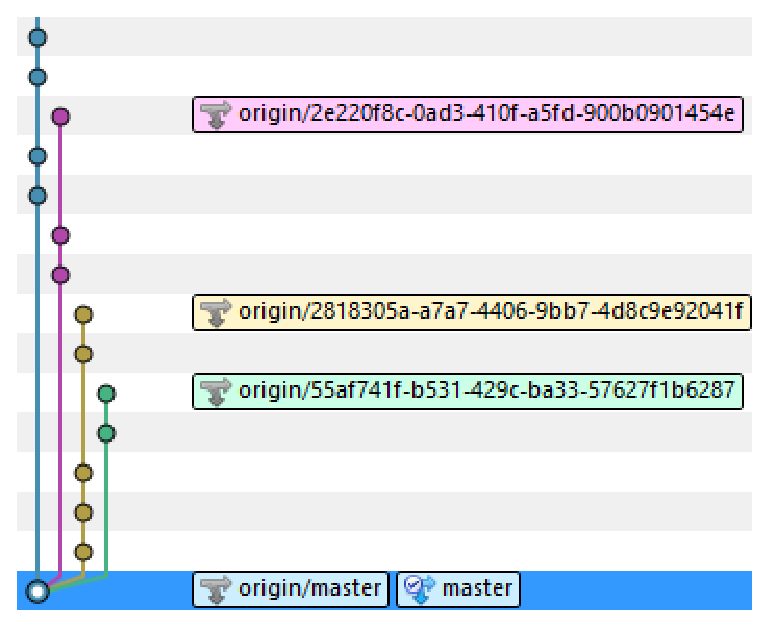
\includegraphics[scale=0.75]{images/tree.eps}
    \caption{Branches du dépôt Git central}
    \label{gitBranch}
\end{center}
\end{figure}

\subsection[Identification des utilisateurs]{Identification des utilisateurs \hyperref[identifPb]{$\uparrow$}}
\label{identifSol}

Le but initial de notre PIDR est de permettre aux professeurs de suivre l'avancement de leurs élèves. Il faut donc pouvoir les identifier sans compromettre leur identité sur le dépôt central. Nous avons donc décider d'utiliser un serveur Play\cite{PlaySite} pour centraliser les données authentifiantes.

\begin{figure}[!h]
\begin{center}
	
\begin{tikzpicture}
\node[server](PC1) at (-3,-1) {};
\node[xshift=-0.8cm,yshift=0.2cm,left of = PC1,align=left](PC1label) {Utilisateur A};

\node(GitA1) at (-5,-2.5) {
\includegraphics[scale=0.25]{images/git.ps}}; 
\node[below of = GitA1,align=left](GitAlabel1) {Git local A1};

\node(GitA2) at (-2,-2.5) {
\includegraphics[scale=0.25]{images/git.ps}}; 
\node[below of = GitA2,align=left](GitAlabel2) {Git local A2};

\node[server](PC2) at (3,-1) {};
\node[xshift=-0.8cm,yshift=0.2cm,left of = PC2,align=left](PC2label) {Utilisateur B};

\node(GitB) at (3,-2.5) {
\includegraphics[scale=0.25]{images/git.ps}}; 
\node[xshift=-0.5cm,left of = GitB,align=left](GitBlabel) {Git local B};
\node[red,inner sep=0mm](croix) at (1.3,0.8) {\begin{LARGE}$\times$\end{LARGE}};

\node[server](PC3) at (4.5,0.5) {};
\node[xshift=0.6cm,right of = PC3,align=left](PC3label) {Utilisateur C};

\node(GitC) at (5.5,-0.5) {
\includegraphics[scale=0.25]{images/git.ps}}; 
\node[xshift=0.7cm,right of = GitC,align=left](GitClabel) {Git local C};


\node[my cloud, minimum width=1.25cm, minimum height=1.55cm,font=\large] (cloud) at (0,2) {Internet};

\node(Git) at (-3.5,3) {
\includegraphics[scale=0.5]{images/git.ps}}; 
\node[xshift=-1cm,left of = Git,align=left](Gitlabel) {Git central};

\node(Play) at (3.5,4) {
\includegraphics[scale=0.15]{images/play.eps}}; 
\node[above of = Play,align=left](Playlabel) {Serveur Play};

\node[server](PCprof) at (6.2,4) {};
\node[xshift=0.8cm,right of = PCprof,align=left](PCproflabel) {Poste professeur};

\draw[thick,darkgray!10!gray] (PC1.north west)--(cloud);
\draw[thick,darkgray!10!gray] (PC1.south east)--(GitA1);
\draw[thick,darkgray!10!gray] (PC1.south west)--(GitA2);
\draw[thick,darkgray!10!gray] (PC2.north east)--(1.3,0.8);
\draw[thick,darkgray!10!gray] (PC2.south)--(GitB);
\draw[thick,darkgray!10!gray] (PC3.north east)--(cloud);
\draw[thick,darkgray!10!gray] (PC3.south)--(GitC);
\draw[thick,darkgray!10!gray] (Git.east)--(cloud);
\draw[thick,darkgray!10!gray] (Play.south west)--(cloud);
\draw[thick,darkgray!10!gray] (Play.east)--(PCprof);
\path[->, red,line width = 0.5mm] (Git)  edge   [bend left=-20]   node {} (Play);
\path[<->, blue,line width = 0.5mm] (GitA2)  edge   [bend left=-80]   node {} (Git.east);
\path[->, darkgray!90,line width = 0.5mm] (PC3) edge [bend left=70] node{} (Play.south west);

\path[<->, blue,line width = 0.5mm] (-4.5,-5)  edge [auto]  node {Git push/pull} (-2,-5);
\path[->, red,line width = 0.5mm] (0,-5)  edge [auto]  node {Git pull} (2.5,-5);
\path[->, darkgray!90,line width = 0.5mm] (4.5,-5)  edge [auto]  node {Liaison d'identité} (7,-5);
\end{tikzpicture}

    \caption{Schéma global}
    \label{schemaGlobal}
\end{center}
\end{figure}


Les élèves seront invités par leur professeur à se connecter sur un serveur Play. Ils devront alors renseigner leur nom, prénom, adresse mail et classe par exemple.

Cela permet de s'assurer que chaque utilisateur \og anonyme\fg{} créé au lancement de la PLM le restera jusqu'au moment où l'utilisateur voudra lier son identité réelle à son identité anonyme. Ce lien se fera sous la forme d'une requête au serveur qui stockera dans une base de données le nom réel, l'adresse mail et le hashé de l'UUID fourni par l'utilisateur afin de savoir à quel utilisateur appartient telle branche vu qu'il n'y a pas d'informations personnelles stockées sur le dépôt distant.

Le reste du PIDR nous ayant déjà demandé beaucoup de temps, le serveur Play ne se trouve pas dans un état très avancé à la fin du projet et ne permet que de pull le dépôt Git central et de consulter la base de données des utilisateurs ayant lié leur identité. Cela pose néanmoins les bases de ce qu'il sera possible de réaliser à l'avenir, comme par exemple offrir aux professeurs une interface web permettant de gérer leurs groupes d'élèves par matière. Voir la figure~\ref{schemaGlobal}.

